% Standalone TikZ diagram: simple unity-feedback closed-loop system.
% Compact form — labels omit the "(s)" suffix for cleaner reading
% (useful in slides, posters, or block-structure illustrations where
% the Laplace-domain context is already established).
% Build:  pdflatex closed_loop_compact.tex

\documentclass[border=4pt]{standalone}
\usepackage{tikz}
\usetikzlibrary{positioning, calc, arrows.meta}

\begin{document}
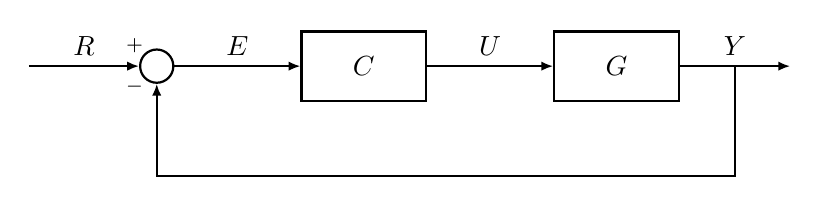
\begin{tikzpicture}[
  >={Latex[length=1.5mm, width=1.2mm]}, thick,
  block/.style = {draw, rectangle, minimum height=2.5em, minimum width=4.5em},
  sum/.style   = {draw, circle, inner sep=0pt, minimum size=1.2em},
]
  \node[coordinate]                    (rin)   {};
  \node[sum,   right=1.4cm of rin]     (sum)   {};
  \node[block, right=1.6cm of sum]     (C)     {$C$};
  \node[block, right=1.6cm of C]       (G)     {$G$};
  \node[coordinate, right=1.4cm of G]  (yout)  {};

  \node[font=\scriptsize, inner sep=0pt, anchor=south east] at (sum.north west) {$+$};
  \node[font=\scriptsize, inner sep=0pt, anchor=north east] at (sum.south west) {$-$};

  \draw[->] (rin) -- node[above]{$R$} (sum);
  \draw[->] (sum) -- node[above]{$E$} (C);
  \draw[->] (C)   -- node[above]{$U$} (G);
  \draw[->] (G)   -- node[above]{$Y$} (yout);

  \coordinate (fbk) at ($(G.east)!0.5!(yout)$);
  \draw[->] (fbk) -- ++(0,-1.4) -| (sum.south);
\end{tikzpicture}
\end{document}
